\documentclass{beamer}
\usepackage{graphicx}
\usepackage{booktabs}
\usepackage{hyperref}
\usepackage{comment}
\usetheme{Madrid}

\title[]{Cumulative Reasoning with Large Language Models}
\subtitle{by Yifan Zhang, Jingqin Yang, Yang Yuan, Andrew Chi-Chih Yao}
\author{Peer Niklas Schäfer}
\institute{University of Cologne}
\date{18.06.2025}

\begin{document}

\begin{frame}
    \titlepage
\end{frame}

%-------------------------------

\begin{frame}{Architecture Overview}
    \begin{figure}
        \centering
        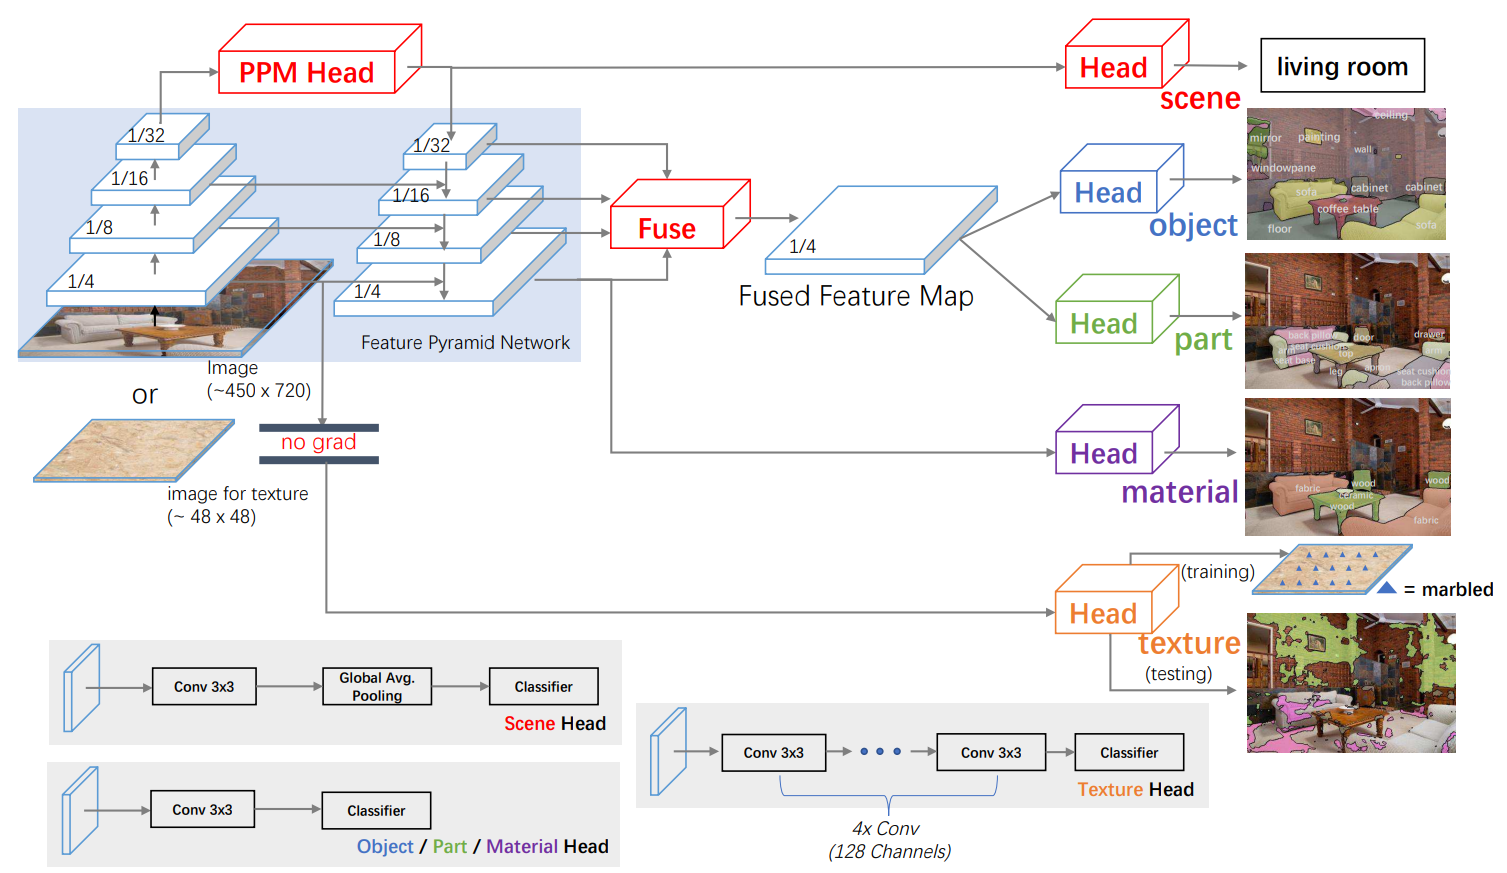
\includegraphics[width=\textwidth]{Images/UPerNetArchitectureOverview.png}

        \vspace{0.5em}
        {\tiny Xiao et al. (2018) ECCV, p. 7}
    \end{figure}
\end{frame}

%-------------------------------

\begin{frame}{Feature Pyramid Networks (FPN)}
    \begin{figure}
        \centering
        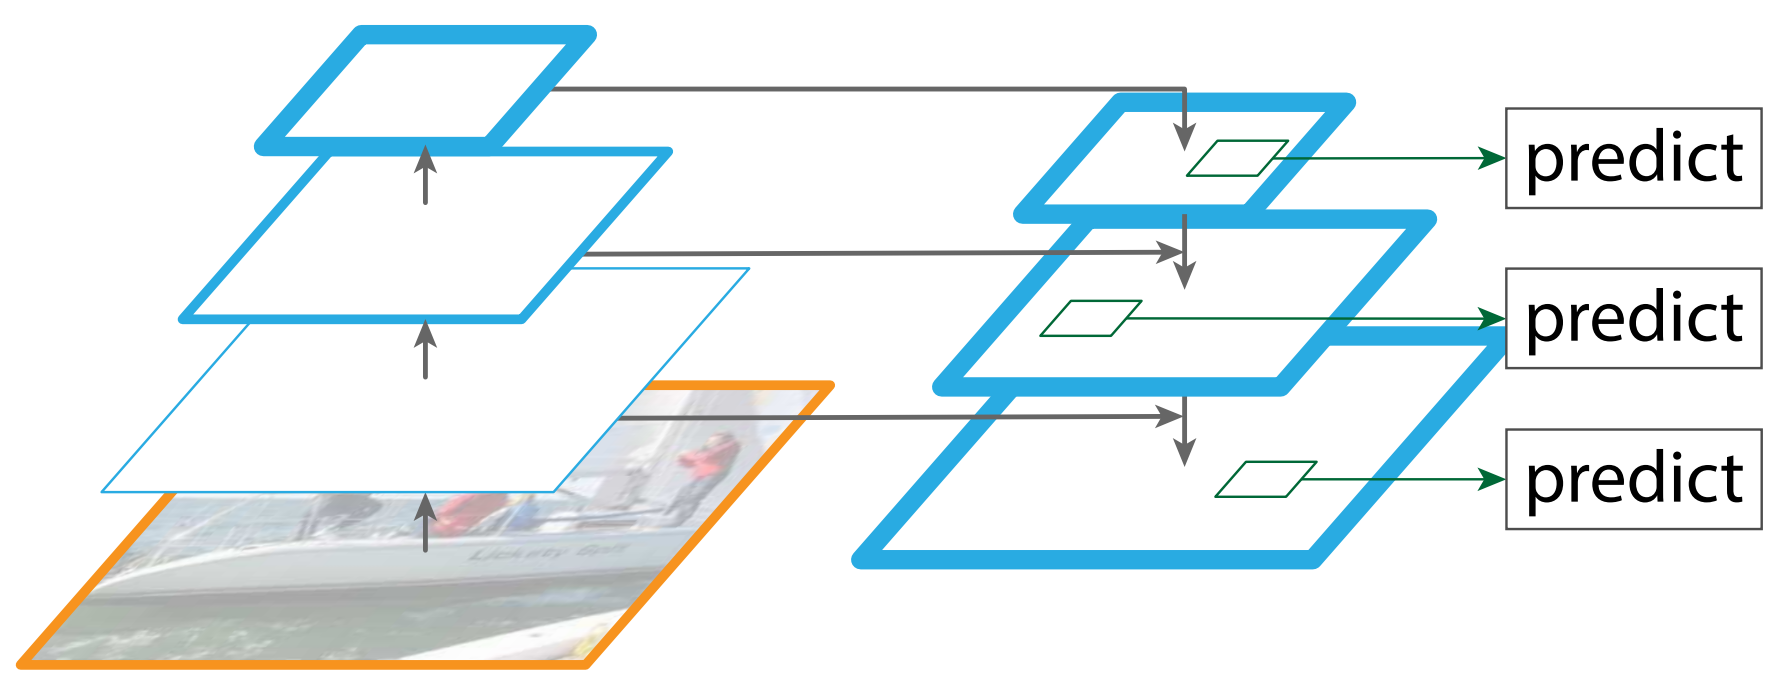
\includegraphics[width=0.7\textwidth]{Images/FPNOverview.png}

        \vspace{0.5em}
        {\tiny Lin et al. (2017) Proceedings of the IEEE conference on computer vision and pattern recognition, p. 2118}
    \end{figure}
    \begin{itemize}
        \item \textbf{Bottom-up pathway:} Computes feature maps at different scales using a convolutional NN
        \item \textbf{Top-down pathway:} Upsamples high-level feature maps back to original size (nearest neighbour upsampling)
        \item \textbf{Lateral connections:} Merges feature maps of \textbf{Top-down pathway} with \textbf{Bottom-up pathway} from same level in hierarchy
    \end{itemize}
\end{frame}

%-------------------------------

\begin{frame}{Architecture Overview}
    \begin{figure}
        \centering
        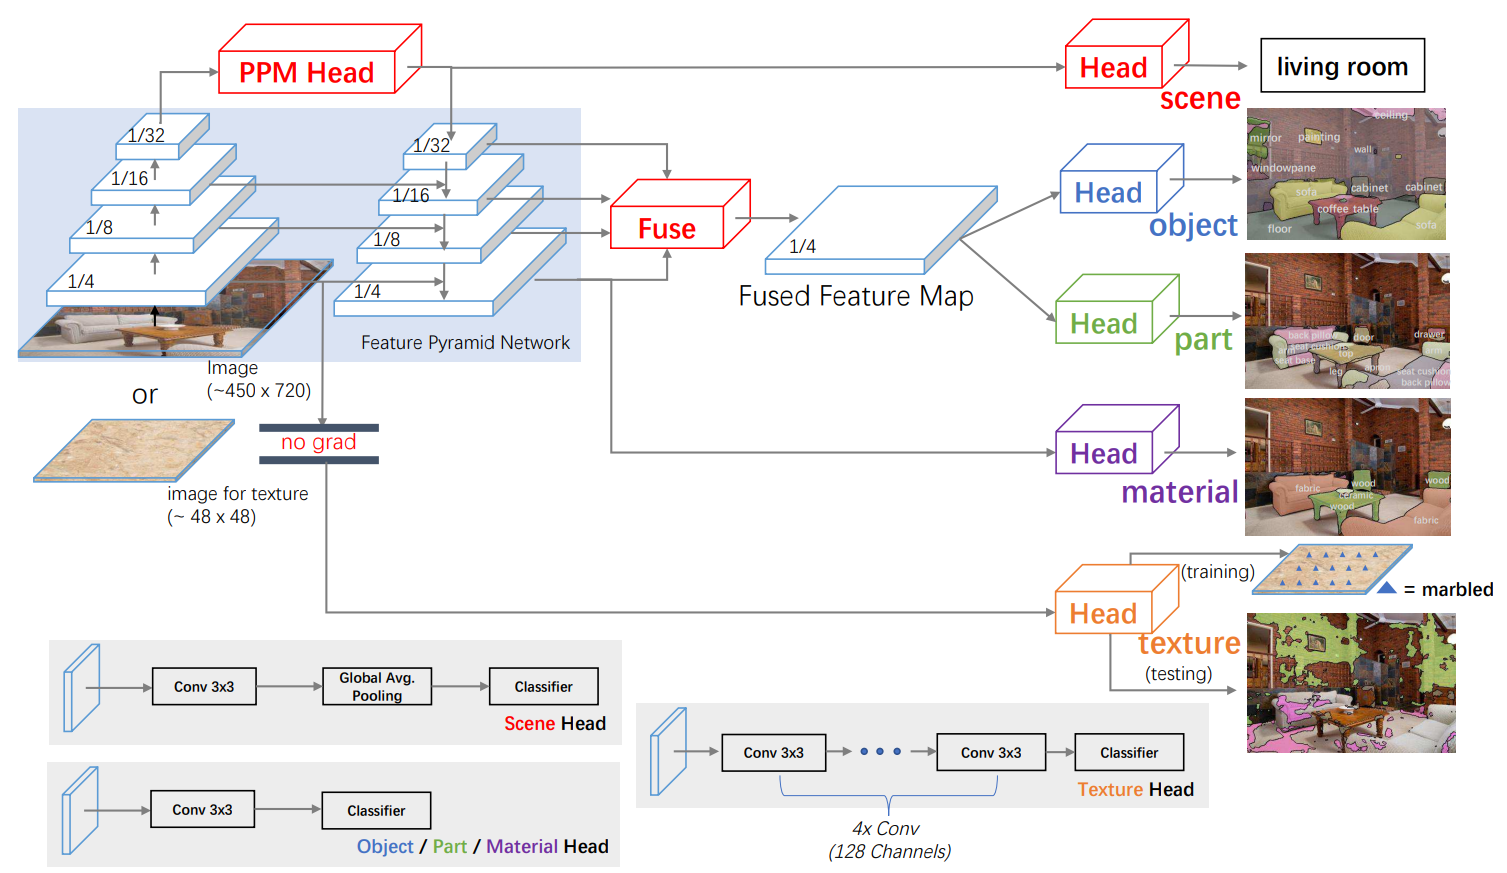
\includegraphics[width=\textwidth]{Images/UPerNetArchitectureOverview.png}

        \vspace{0.5em}
        {\tiny Xiao et al. (2018) ECCV, p. 7}
    \end{figure}
\end{frame}

%-------------------------------

\begin{frame}{PPM Module}
    \begin{figure}
        \centering
        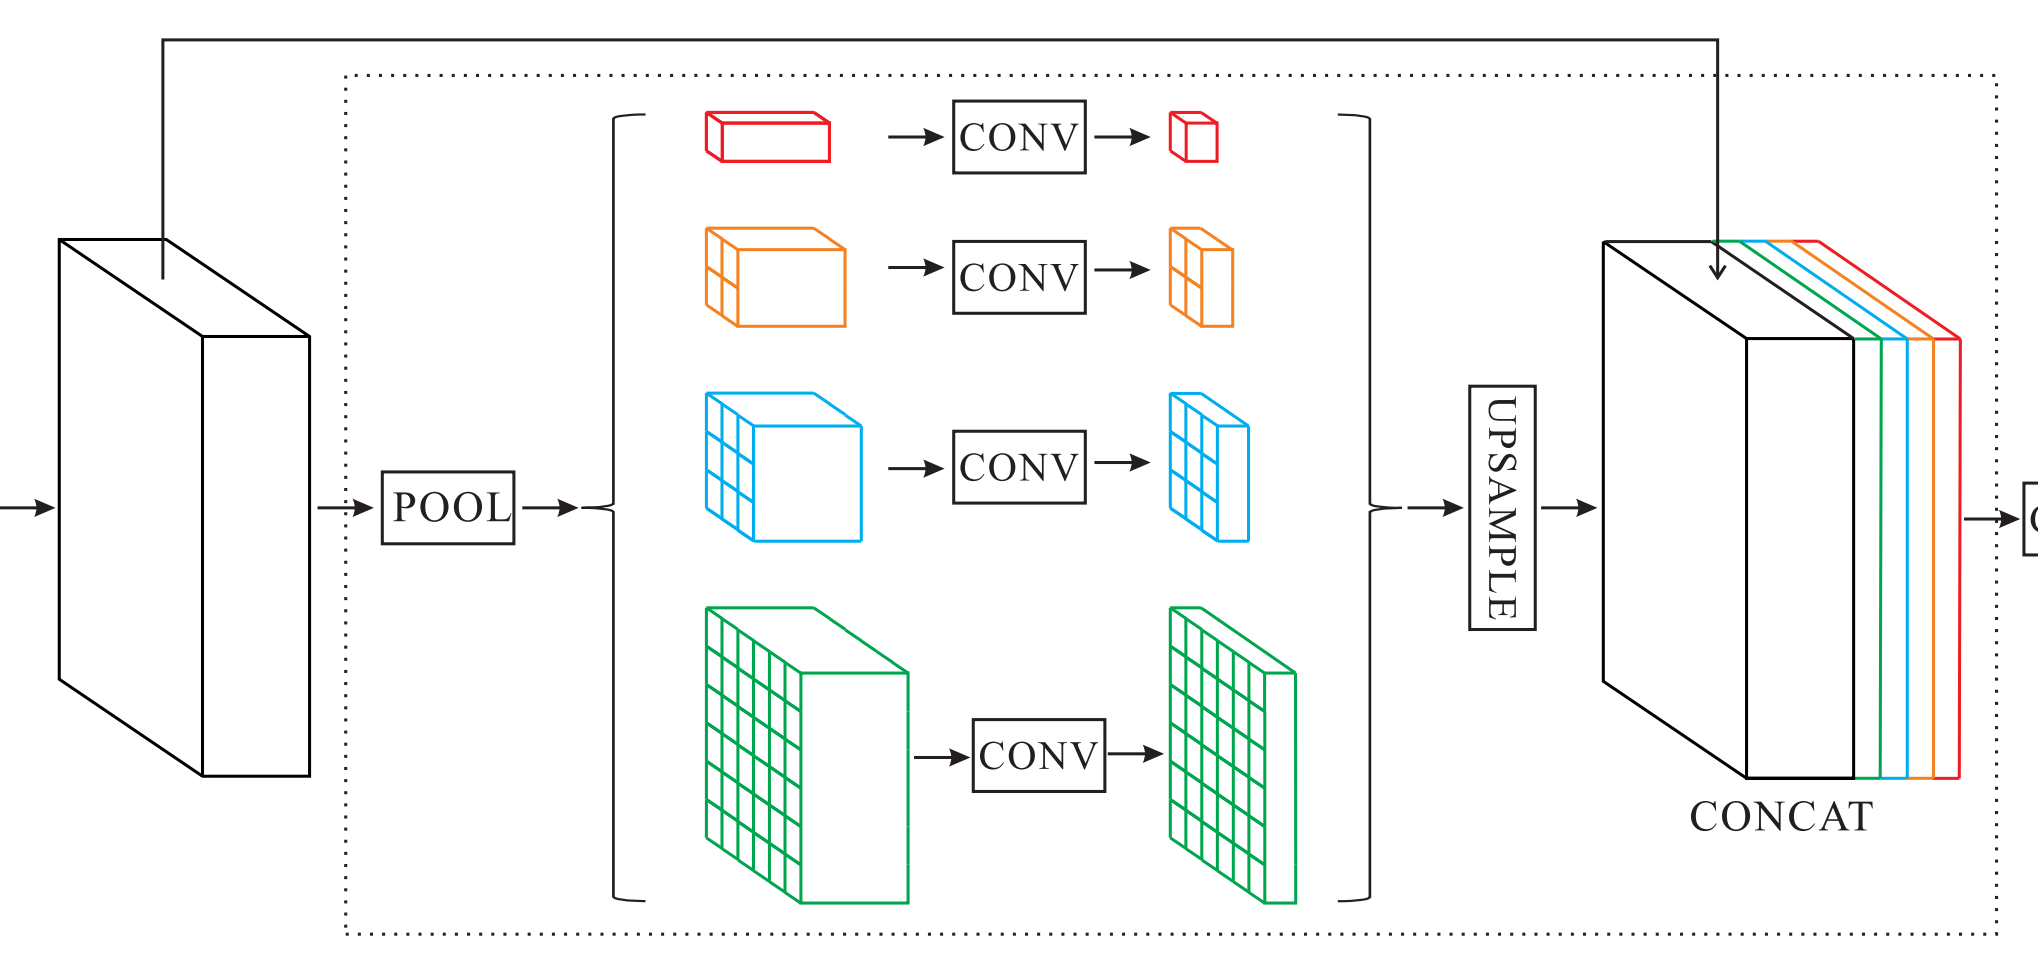
\includegraphics[width=0.7\textwidth]{Images/PPMModuleOverview.png}

        %\vspace{0.5em}
        {\tiny Zhao et al. (2017) IEEE conference on computer vision and pattern recognition, p. 2884}
    \end{figure}
    \begin{itemize}
        \item Input is a feature map provided by some CNN
        \item Different pooling operations produce different sized feature maps
        \item Reduce dimensionality with a 1x1 convolution
        \item Upsample via interpolation to original size
        \item Concatenate results with original feature map
        \item PPM is used to address limited receptive field of deep CNNs
    \end{itemize}
\end{frame}

%-------------------------------

\begin{frame}{Architecture Overview}
    \begin{figure}
        \centering
        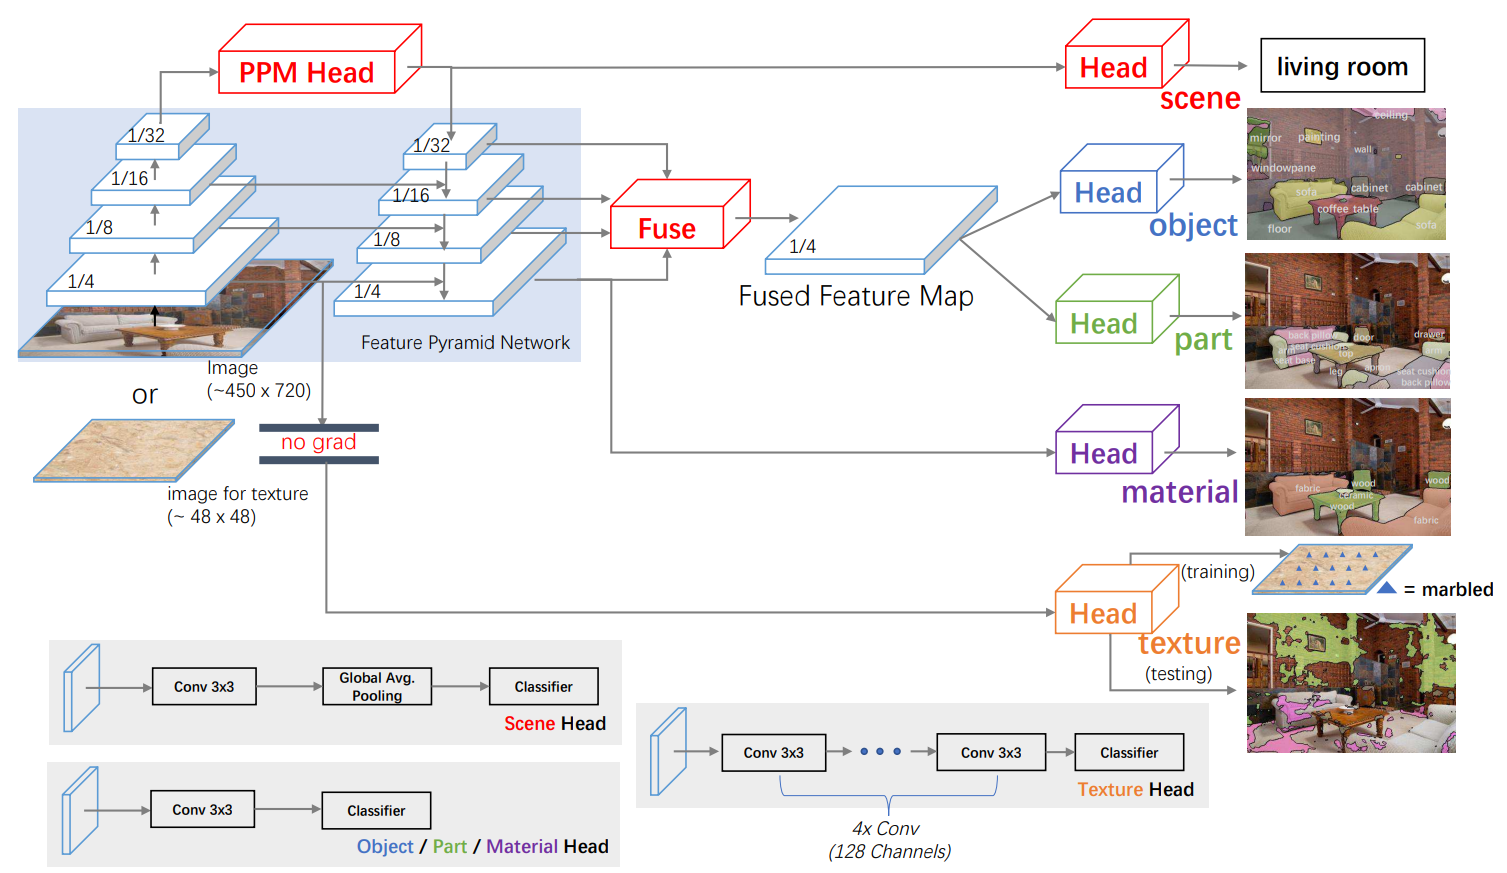
\includegraphics[width=\textwidth]{Images/UPerNetArchitectureOverview.png}

        \vspace{0.5em}
        {\tiny Xiao et al. (2018) ECCV, p. 7}
    \end{figure}
\end{frame}

%-------------------------------

\begin{comment}
\item Every classifier is preceded by a separate convolutional head. To fuse the layers
with different scales such as {P2, P3, P4, P5}, we resize them via bilinear interpolation to the size of P2 and concatenate these layers. A convolutional layer
is then applied to fuse features from different levels as well as to reduce channel dimensions
\item To overcome the issue raised by Zhou et
al. [32] that although the theoretical receptive field of deep CNN is large enough,
the empirical receptive field of deep CNN is relatively much smaller [33], we apply a Pyramid Pooling Module (PPM) from PSPNet [16] on the last layer of the
backbone network before feeding it into the top-down branch in FPN. Empirically we find that the PPM is highly compatible with the FPN architecture by
bringing effective global prior representations.
\item Scene label, the highest-level
attribute annotated at image-level, is predicted by a global average pooling of P5
8 T. Xiao, Y. Liu, B. Zhou, Y. Jiang, J. Sun
followed by a linear classifier.
\item For object label,
we empirically find that fusing all feature maps of FPN is better than only using
the feature map with the highest resolution (P2). Object parts are segmented
based on the same feature map as objects.
\item For materials, intuitively, if we have
prior knowledge that these areas belong to the object “cup”, we are able to
make a reasonable conjecture that it might be made up of paper or plastics.
This context is useful, but we still need local apparent features to decide which
one is correct. It should also be noted that an object can be made up of various
materials. Based on the above observations, we segment materials on top of P2
rather than fused features.
\item Texture label, given at the image-level, is based on
non-natural images. Directly fusing these images with other natural images is
harmful to other tasks. Also we hope the network can predict texture labels at
pixel level. To achieve such a goal, we append several convolutional layers on
top of C2, and force the network to predict the texture label at every pixel.
The gradient of this branch is prevented from back-propagating to layers of
backbone networks, and the training images for texture are resized to a smaller
size (∼ 64 × 64). The reasons behind these designs are: 1) Texture is the lowestlevel perceptual attribute, thus it is purely based on apparent features and does
not need any high-level information. 2) Essential features for predicting texture
correctly are implicitly learned when trained on other tasks. 3) The receptive
field of this branch needs to be small enough, so that the network is able to
predict different labels at various regions when an image at normal scale is fed
in the network. We only fine-tune the texture branch for a few epochs after the
whole network finishes training on other tasks.
\end{comment}

\begin{frame}{Notes}
    \begin{itemize}
        \item Every classifier is preceded by a separate convolutional head.
        \item Fusing feature maps is done via bilinear interpolation.
        \item Scene labels are predicted using global average pooling on high-level features (P5).
        \item Object and part segmentation benefits from fusing all FPN feature maps, not just the highest resolution.
        \item Material segmentation is performed on P2 features, leveraging both context and local appearance.
        \item Texture labels are predicted at pixel level using a dedicated branch on low-level features (C2), with training isolated from the main backbone.
    \end{itemize}
\end{frame}

%-------------------------------

\begin{frame}{Sources}
    \begin{itemize}
        \item XIAO, Tete, et al. Unified perceptual parsing for scene understanding. In: Proceedings of the European conference on computer vision (ECCV). 2018. S. 418-434.
        \item LIN, Tsung-Yi, et al. Feature pyramid networks for object detection. In: Proceedings of the IEEE conference on computer vision and pattern recognition. 2017. S. 2117-2125.materials
        \item ZHAO, Hengshuang, et al. Pyramid scene parsing network. In: Proceedings of the IEEE conference on computer vision and pattern recognition. 2017. S. 2881-2890.
    \end{itemize}
\end{frame}

\end{document}
